% Created by tikzDevice version 0.10.1 on 2016-11-20 17:29:55
% !TEX encoding = UTF-8 Unicode
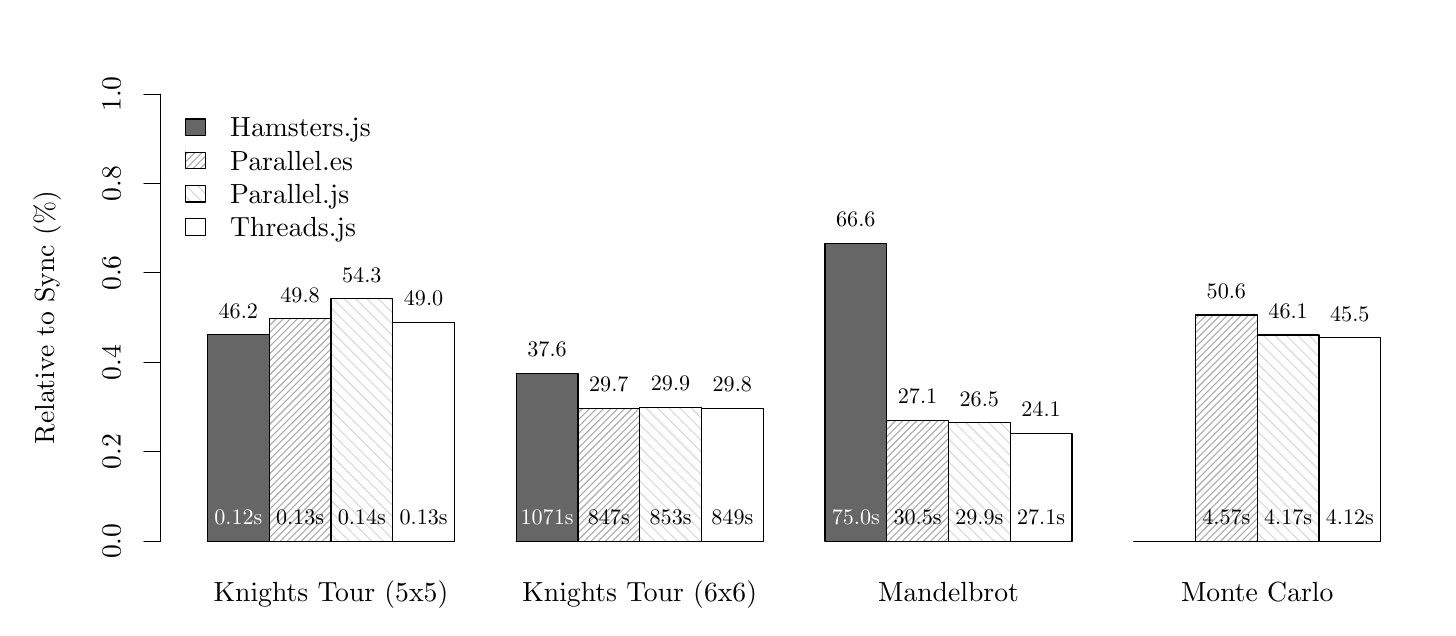
\begin{tikzpicture}[x=1pt,y=1pt]
\definecolor{fillColor}{RGB}{255,255,255}
\path[use as bounding box,fill=fillColor,fill opacity=0.00] (0,0) rectangle (505.89,209.58);
\begin{scope}
\path[clip] (  0.00,  0.00) rectangle (505.89,209.58);
\definecolor{fillColor}{gray}{0.40}

\path[fill=fillColor] ( 64.96, 24.00) --
	( 87.27, 24.00) --
	( 87.27, 98.59) --
	( 64.96, 98.59) --
	cycle;
\definecolor{drawColor}{RGB}{172,172,172}

\path[draw=drawColor,line width= 0.4pt,line join=round,line cap=round] ( 87.27,104.40) -- ( 87.28,104.41);

\path[draw=drawColor,line width= 0.4pt,line join=round,line cap=round] ( 87.27,101.85) -- ( 89.84,104.41);

\path[draw=drawColor,line width= 0.4pt,line join=round,line cap=round] ( 87.27, 99.29) -- ( 92.39,104.41);

\path[draw=drawColor,line width= 0.4pt,line join=round,line cap=round] ( 87.27, 96.74) -- ( 94.95,104.41);

\path[draw=drawColor,line width= 0.4pt,line join=round,line cap=round] ( 87.27, 94.18) -- ( 97.50,104.41);

\path[draw=drawColor,line width= 0.4pt,line join=round,line cap=round] ( 87.27, 91.62) -- (100.06,104.41);

\path[draw=drawColor,line width= 0.4pt,line join=round,line cap=round] ( 87.27, 89.07) -- (102.61,104.41);

\path[draw=drawColor,line width= 0.4pt,line join=round,line cap=round] ( 87.27, 86.51) -- (105.17,104.41);

\path[draw=drawColor,line width= 0.4pt,line join=round,line cap=round] ( 87.27, 83.96) -- (107.72,104.41);

\path[draw=drawColor,line width= 0.4pt,line join=round,line cap=round] ( 87.27, 81.40) -- (109.59,103.72);

\path[draw=drawColor,line width= 0.4pt,line join=round,line cap=round] ( 87.27, 78.85) -- (109.59,101.16);

\path[draw=drawColor,line width= 0.4pt,line join=round,line cap=round] ( 87.27, 76.29) -- (109.59, 98.61);

\path[draw=drawColor,line width= 0.4pt,line join=round,line cap=round] ( 87.27, 73.74) -- (109.59, 96.05);

\path[draw=drawColor,line width= 0.4pt,line join=round,line cap=round] ( 87.27, 71.18) -- (109.59, 93.50);

\path[draw=drawColor,line width= 0.4pt,line join=round,line cap=round] ( 87.27, 68.63) -- (109.59, 90.94);

\path[draw=drawColor,line width= 0.4pt,line join=round,line cap=round] ( 87.27, 66.07) -- (109.59, 88.39);

\path[draw=drawColor,line width= 0.4pt,line join=round,line cap=round] ( 87.27, 63.52) -- (109.59, 85.83);

\path[draw=drawColor,line width= 0.4pt,line join=round,line cap=round] ( 87.27, 60.96) -- (109.59, 83.28);

\path[draw=drawColor,line width= 0.4pt,line join=round,line cap=round] ( 87.27, 58.41) -- (109.59, 80.72);

\path[draw=drawColor,line width= 0.4pt,line join=round,line cap=round] ( 87.27, 55.85) -- (109.59, 78.17);

\path[draw=drawColor,line width= 0.4pt,line join=round,line cap=round] ( 87.27, 53.30) -- (109.59, 75.61);

\path[draw=drawColor,line width= 0.4pt,line join=round,line cap=round] ( 87.27, 50.74) -- (109.59, 73.06);

\path[draw=drawColor,line width= 0.4pt,line join=round,line cap=round] ( 87.27, 48.19) -- (109.59, 70.50);

\path[draw=drawColor,line width= 0.4pt,line join=round,line cap=round] ( 87.27, 45.63) -- (109.59, 67.95);

\path[draw=drawColor,line width= 0.4pt,line join=round,line cap=round] ( 87.27, 43.08) -- (109.59, 65.39);

\path[draw=drawColor,line width= 0.4pt,line join=round,line cap=round] ( 87.27, 40.52) -- (109.59, 62.84);

\path[draw=drawColor,line width= 0.4pt,line join=round,line cap=round] ( 87.27, 37.97) -- (109.59, 60.28);

\path[draw=drawColor,line width= 0.4pt,line join=round,line cap=round] ( 87.27, 35.41) -- (109.59, 57.73);

\path[draw=drawColor,line width= 0.4pt,line join=round,line cap=round] ( 87.27, 32.86) -- (109.59, 55.17);

\path[draw=drawColor,line width= 0.4pt,line join=round,line cap=round] ( 87.27, 30.30) -- (109.59, 52.62);

\path[draw=drawColor,line width= 0.4pt,line join=round,line cap=round] ( 87.27, 27.75) -- (109.59, 50.06);

\path[draw=drawColor,line width= 0.4pt,line join=round,line cap=round] ( 87.27, 25.19) -- (109.59, 47.51);

\path[draw=drawColor,line width= 0.4pt,line join=round,line cap=round] ( 88.64, 24.00) -- (109.59, 44.95);

\path[draw=drawColor,line width= 0.4pt,line join=round,line cap=round] ( 91.19, 24.00) -- (109.59, 42.40);

\path[draw=drawColor,line width= 0.4pt,line join=round,line cap=round] ( 93.75, 24.00) -- (109.59, 39.84);

\path[draw=drawColor,line width= 0.4pt,line join=round,line cap=round] ( 96.30, 24.00) -- (109.59, 37.29);

\path[draw=drawColor,line width= 0.4pt,line join=round,line cap=round] ( 98.86, 24.00) -- (109.59, 34.73);

\path[draw=drawColor,line width= 0.4pt,line join=round,line cap=round] (101.41, 24.00) -- (109.59, 32.17);

\path[draw=drawColor,line width= 0.4pt,line join=round,line cap=round] (103.97, 24.00) -- (109.59, 29.62);

\path[draw=drawColor,line width= 0.4pt,line join=round,line cap=round] (106.52, 24.00) -- (109.59, 27.06);

\path[draw=drawColor,line width= 0.4pt,line join=round,line cap=round] (109.08, 24.00) -- (109.59, 24.51);
\definecolor{drawColor}{RGB}{218,218,218}

\path[draw=drawColor,line width= 0.4pt,line join=round,line cap=round] (112.14, 24.00) -- (109.59, 26.56);

\path[draw=drawColor,line width= 0.4pt,line join=round,line cap=round] (116.23, 24.00) -- (109.59, 30.64);

\path[draw=drawColor,line width= 0.4pt,line join=round,line cap=round] (120.32, 24.00) -- (109.59, 34.73);

\path[draw=drawColor,line width= 0.4pt,line join=round,line cap=round] (124.41, 24.00) -- (109.59, 38.82);

\path[draw=drawColor,line width= 0.4pt,line join=round,line cap=round] (128.50, 24.00) -- (109.59, 42.91);

\path[draw=drawColor,line width= 0.4pt,line join=round,line cap=round] (131.90, 24.68) -- (109.59, 47.00);

\path[draw=drawColor,line width= 0.4pt,line join=round,line cap=round] (131.90, 28.77) -- (109.59, 51.09);

\path[draw=drawColor,line width= 0.4pt,line join=round,line cap=round] (131.90, 32.86) -- (109.59, 55.17);

\path[draw=drawColor,line width= 0.4pt,line join=round,line cap=round] (131.90, 36.95) -- (109.59, 59.26);

\path[draw=drawColor,line width= 0.4pt,line join=round,line cap=round] (131.90, 41.04) -- (109.59, 63.35);

\path[draw=drawColor,line width= 0.4pt,line join=round,line cap=round] (131.90, 45.12) -- (109.59, 67.44);

\path[draw=drawColor,line width= 0.4pt,line join=round,line cap=round] (131.90, 49.21) -- (109.59, 71.53);

\path[draw=drawColor,line width= 0.4pt,line join=round,line cap=round] (131.90, 53.30) -- (109.59, 75.62);

\path[draw=drawColor,line width= 0.4pt,line join=round,line cap=round] (131.90, 57.39) -- (109.59, 79.70);

\path[draw=drawColor,line width= 0.4pt,line join=round,line cap=round] (131.90, 61.48) -- (109.59, 83.79);

\path[draw=drawColor,line width= 0.4pt,line join=round,line cap=round] (131.90, 65.57) -- (109.59, 87.88);

\path[draw=drawColor,line width= 0.4pt,line join=round,line cap=round] (131.90, 69.65) -- (109.59, 91.97);

\path[draw=drawColor,line width= 0.4pt,line join=round,line cap=round] (131.90, 73.74) -- (109.59, 96.06);

\path[draw=drawColor,line width= 0.4pt,line join=round,line cap=round] (131.90, 77.83) -- (109.59,100.14);

\path[draw=drawColor,line width= 0.4pt,line join=round,line cap=round] (131.90, 81.92) -- (109.59,104.23);

\path[draw=drawColor,line width= 0.4pt,line join=round,line cap=round] (131.90, 86.01) -- (109.59,108.32);

\path[draw=drawColor,line width= 0.4pt,line join=round,line cap=round] (131.90, 90.09) -- (110.33,111.67);

\path[draw=drawColor,line width= 0.4pt,line join=round,line cap=round] (131.90, 94.18) -- (114.42,111.67);

\path[draw=drawColor,line width= 0.4pt,line join=round,line cap=round] (131.90, 98.27) -- (118.50,111.67);

\path[draw=drawColor,line width= 0.4pt,line join=round,line cap=round] (131.90,102.36) -- (122.59,111.67);

\path[draw=drawColor,line width= 0.4pt,line join=round,line cap=round] (131.90,106.45) -- (126.68,111.67);

\path[draw=drawColor,line width= 0.4pt,line join=round,line cap=round] (131.90,110.54) -- (130.77,111.67);

\path[fill=fillColor] (176.53, 24.00) --
	(198.84, 24.00) --
	(198.84, 84.69) --
	(176.53, 84.69) --
	cycle;
\definecolor{drawColor}{RGB}{172,172,172}

\path[draw=drawColor,line width= 0.4pt,line join=round,line cap=round] (198.84, 70.33) -- (200.50, 71.98);

\path[draw=drawColor,line width= 0.4pt,line join=round,line cap=round] (198.84, 67.77) -- (203.05, 71.98);

\path[draw=drawColor,line width= 0.4pt,line join=round,line cap=round] (198.84, 65.22) -- (205.61, 71.98);

\path[draw=drawColor,line width= 0.4pt,line join=round,line cap=round] (198.84, 62.66) -- (208.16, 71.98);

\path[draw=drawColor,line width= 0.4pt,line join=round,line cap=round] (198.84, 60.11) -- (210.72, 71.98);

\path[draw=drawColor,line width= 0.4pt,line join=round,line cap=round] (198.84, 57.55) -- (213.27, 71.98);

\path[draw=drawColor,line width= 0.4pt,line join=round,line cap=round] (198.84, 55.00) -- (215.83, 71.98);

\path[draw=drawColor,line width= 0.4pt,line join=round,line cap=round] (198.84, 52.44) -- (218.39, 71.98);

\path[draw=drawColor,line width= 0.4pt,line join=round,line cap=round] (198.84, 49.89) -- (220.94, 71.98);

\path[draw=drawColor,line width= 0.4pt,line join=round,line cap=round] (198.84, 47.33) -- (221.16, 69.65);

\path[draw=drawColor,line width= 0.4pt,line join=round,line cap=round] (198.84, 44.78) -- (221.16, 67.09);

\path[draw=drawColor,line width= 0.4pt,line join=round,line cap=round] (198.84, 42.22) -- (221.16, 64.54);

\path[draw=drawColor,line width= 0.4pt,line join=round,line cap=round] (198.84, 39.67) -- (221.16, 61.98);

\path[draw=drawColor,line width= 0.4pt,line join=round,line cap=round] (198.84, 37.11) -- (221.16, 59.43);

\path[draw=drawColor,line width= 0.4pt,line join=round,line cap=round] (198.84, 34.56) -- (221.16, 56.87);

\path[draw=drawColor,line width= 0.4pt,line join=round,line cap=round] (198.84, 32.00) -- (221.16, 54.32);

\path[draw=drawColor,line width= 0.4pt,line join=round,line cap=round] (198.84, 29.45) -- (221.16, 51.76);

\path[draw=drawColor,line width= 0.4pt,line join=round,line cap=round] (198.84, 26.89) -- (221.16, 49.21);

\path[draw=drawColor,line width= 0.4pt,line join=round,line cap=round] (198.84, 24.34) -- (221.16, 46.65);

\path[draw=drawColor,line width= 0.4pt,line join=round,line cap=round] (201.06, 24.00) -- (221.16, 44.10);

\path[draw=drawColor,line width= 0.4pt,line join=round,line cap=round] (203.62, 24.00) -- (221.16, 41.54);

\path[draw=drawColor,line width= 0.4pt,line join=round,line cap=round] (206.17, 24.00) -- (221.16, 38.99);

\path[draw=drawColor,line width= 0.4pt,line join=round,line cap=round] (208.73, 24.00) -- (221.16, 36.43);

\path[draw=drawColor,line width= 0.4pt,line join=round,line cap=round] (211.28, 24.00) -- (221.16, 33.88);

\path[draw=drawColor,line width= 0.4pt,line join=round,line cap=round] (213.84, 24.00) -- (221.16, 31.32);

\path[draw=drawColor,line width= 0.4pt,line join=round,line cap=round] (216.39, 24.00) -- (221.16, 28.77);

\path[draw=drawColor,line width= 0.4pt,line join=round,line cap=round] (218.95, 24.00) -- (221.16, 26.21);
\definecolor{drawColor}{RGB}{218,218,218}

\path[draw=drawColor,line width= 0.4pt,line join=round,line cap=round] (222.53, 24.00) -- (221.16, 25.37);

\path[draw=drawColor,line width= 0.4pt,line join=round,line cap=round] (226.61, 24.00) -- (221.16, 29.45);

\path[draw=drawColor,line width= 0.4pt,line join=round,line cap=round] (230.70, 24.00) -- (221.16, 33.54);

\path[draw=drawColor,line width= 0.4pt,line join=round,line cap=round] (234.79, 24.00) -- (221.16, 37.63);

\path[draw=drawColor,line width= 0.4pt,line join=round,line cap=round] (238.88, 24.00) -- (221.16, 41.72);

\path[draw=drawColor,line width= 0.4pt,line join=round,line cap=round] (242.97, 24.00) -- (221.16, 45.81);

\path[draw=drawColor,line width= 0.4pt,line join=round,line cap=round] (243.47, 27.58) -- (221.16, 49.90);

\path[draw=drawColor,line width= 0.4pt,line join=round,line cap=round] (243.47, 31.67) -- (221.16, 53.98);

\path[draw=drawColor,line width= 0.4pt,line join=round,line cap=round] (243.47, 35.76) -- (221.16, 58.07);

\path[draw=drawColor,line width= 0.4pt,line join=round,line cap=round] (243.47, 39.85) -- (221.16, 62.16);

\path[draw=drawColor,line width= 0.4pt,line join=round,line cap=round] (243.47, 43.93) -- (221.16, 66.25);

\path[draw=drawColor,line width= 0.4pt,line join=round,line cap=round] (243.47, 48.02) -- (221.16, 70.34);

\path[draw=drawColor,line width= 0.4pt,line join=round,line cap=round] (243.47, 52.11) -- (223.24, 72.34);

\path[draw=drawColor,line width= 0.4pt,line join=round,line cap=round] (243.47, 56.20) -- (227.33, 72.34);

\path[draw=drawColor,line width= 0.4pt,line join=round,line cap=round] (243.47, 60.29) -- (231.42, 72.34);

\path[draw=drawColor,line width= 0.4pt,line join=round,line cap=round] (243.47, 64.38) -- (235.51, 72.34);

\path[draw=drawColor,line width= 0.4pt,line join=round,line cap=round] (243.47, 68.46) -- (239.60, 72.34);

\path[fill=fillColor] (288.10, 24.00) --
	(310.42, 24.00) --
	(310.42,131.63) --
	(288.10,131.63) --
	cycle;
\definecolor{drawColor}{RGB}{172,172,172}

\path[draw=drawColor,line width= 0.4pt,line join=round,line cap=round] (310.42, 66.92) -- (311.23, 67.73);

\path[draw=drawColor,line width= 0.4pt,line join=round,line cap=round] (310.42, 64.37) -- (313.78, 67.73);

\path[draw=drawColor,line width= 0.4pt,line join=round,line cap=round] (310.42, 61.81) -- (316.34, 67.73);

\path[draw=drawColor,line width= 0.4pt,line join=round,line cap=round] (310.42, 59.26) -- (318.89, 67.73);

\path[draw=drawColor,line width= 0.4pt,line join=round,line cap=round] (310.42, 56.70) -- (321.45, 67.73);

\path[draw=drawColor,line width= 0.4pt,line join=round,line cap=round] (310.42, 54.14) -- (324.00, 67.73);

\path[draw=drawColor,line width= 0.4pt,line join=round,line cap=round] (310.42, 51.59) -- (326.56, 67.73);

\path[draw=drawColor,line width= 0.4pt,line join=round,line cap=round] (310.42, 49.03) -- (329.11, 67.73);

\path[draw=drawColor,line width= 0.4pt,line join=round,line cap=round] (310.42, 46.48) -- (331.67, 67.73);

\path[draw=drawColor,line width= 0.4pt,line join=round,line cap=round] (310.42, 43.92) -- (332.73, 66.24);

\path[draw=drawColor,line width= 0.4pt,line join=round,line cap=round] (310.42, 41.37) -- (332.73, 63.68);

\path[draw=drawColor,line width= 0.4pt,line join=round,line cap=round] (310.42, 38.81) -- (332.73, 61.13);

\path[draw=drawColor,line width= 0.4pt,line join=round,line cap=round] (310.42, 36.26) -- (332.73, 58.57);

\path[draw=drawColor,line width= 0.4pt,line join=round,line cap=round] (310.42, 33.70) -- (332.73, 56.02);

\path[draw=drawColor,line width= 0.4pt,line join=round,line cap=round] (310.42, 31.15) -- (332.73, 53.46);

\path[draw=drawColor,line width= 0.4pt,line join=round,line cap=round] (310.42, 28.59) -- (332.73, 50.91);

\path[draw=drawColor,line width= 0.4pt,line join=round,line cap=round] (310.42, 26.04) -- (332.73, 48.35);

\path[draw=drawColor,line width= 0.4pt,line join=round,line cap=round] (310.93, 24.00) -- (332.73, 45.80);

\path[draw=drawColor,line width= 0.4pt,line join=round,line cap=round] (313.49, 24.00) -- (332.73, 43.24);

\path[draw=drawColor,line width= 0.4pt,line join=round,line cap=round] (316.04, 24.00) -- (332.73, 40.69);

\path[draw=drawColor,line width= 0.4pt,line join=round,line cap=round] (318.60, 24.00) -- (332.73, 38.13);

\path[draw=drawColor,line width= 0.4pt,line join=round,line cap=round] (321.15, 24.00) -- (332.73, 35.58);

\path[draw=drawColor,line width= 0.4pt,line join=round,line cap=round] (323.71, 24.00) -- (332.73, 33.02);

\path[draw=drawColor,line width= 0.4pt,line join=round,line cap=round] (326.26, 24.00) -- (332.73, 30.47);

\path[draw=drawColor,line width= 0.4pt,line join=round,line cap=round] (328.82, 24.00) -- (332.73, 27.91);

\path[draw=drawColor,line width= 0.4pt,line join=round,line cap=round] (331.37, 24.00) -- (332.73, 25.36);
\definecolor{drawColor}{RGB}{218,218,218}

\path[draw=drawColor,line width= 0.4pt,line join=round,line cap=round] (332.91, 24.00) -- (332.73, 24.18);

\path[draw=drawColor,line width= 0.4pt,line join=round,line cap=round] (337.00, 24.00) -- (332.73, 28.26);

\path[draw=drawColor,line width= 0.4pt,line join=round,line cap=round] (341.08, 24.00) -- (332.73, 32.35);

\path[draw=drawColor,line width= 0.4pt,line join=round,line cap=round] (345.17, 24.00) -- (332.73, 36.44);

\path[draw=drawColor,line width= 0.4pt,line join=round,line cap=round] (349.26, 24.00) -- (332.73, 40.53);

\path[draw=drawColor,line width= 0.4pt,line join=round,line cap=round] (353.35, 24.00) -- (332.73, 44.62);

\path[draw=drawColor,line width= 0.4pt,line join=round,line cap=round] (355.05, 26.39) -- (332.73, 48.71);

\path[draw=drawColor,line width= 0.4pt,line join=round,line cap=round] (355.05, 30.48) -- (332.73, 52.79);

\path[draw=drawColor,line width= 0.4pt,line join=round,line cap=round] (355.05, 34.57) -- (332.73, 56.88);

\path[draw=drawColor,line width= 0.4pt,line join=round,line cap=round] (355.05, 38.66) -- (332.73, 60.97);

\path[draw=drawColor,line width= 0.4pt,line join=round,line cap=round] (355.05, 42.74) -- (332.73, 65.06);

\path[draw=drawColor,line width= 0.4pt,line join=round,line cap=round] (355.05, 46.83) -- (335.03, 66.85);

\path[draw=drawColor,line width= 0.4pt,line join=round,line cap=round] (355.05, 50.92) -- (339.12, 66.85);

\path[draw=drawColor,line width= 0.4pt,line join=round,line cap=round] (355.05, 55.01) -- (343.21, 66.85);

\path[draw=drawColor,line width= 0.4pt,line join=round,line cap=round] (355.05, 59.10) -- (347.30, 66.85);

\path[draw=drawColor,line width= 0.4pt,line join=round,line cap=round] (355.05, 63.19) -- (351.38, 66.85);

\path[fill=fillColor] (399.67, 24.00) --
	(421.99, 24.00) --
	cycle;
\definecolor{drawColor}{RGB}{172,172,172}

\path[draw=drawColor,line width= 0.4pt,line join=round,line cap=round] (421.99,104.39) -- (423.35,105.75);

\path[draw=drawColor,line width= 0.4pt,line join=round,line cap=round] (421.99,101.84) -- (425.90,105.75);

\path[draw=drawColor,line width= 0.4pt,line join=round,line cap=round] (421.99, 99.28) -- (428.46,105.75);

\path[draw=drawColor,line width= 0.4pt,line join=round,line cap=round] (421.99, 96.73) -- (431.01,105.75);

\path[draw=drawColor,line width= 0.4pt,line join=round,line cap=round] (421.99, 94.17) -- (433.57,105.75);

\path[draw=drawColor,line width= 0.4pt,line join=round,line cap=round] (421.99, 91.62) -- (436.12,105.75);

\path[draw=drawColor,line width= 0.4pt,line join=round,line cap=round] (421.99, 89.06) -- (438.68,105.75);

\path[draw=drawColor,line width= 0.4pt,line join=round,line cap=round] (421.99, 86.51) -- (441.24,105.75);

\path[draw=drawColor,line width= 0.4pt,line join=round,line cap=round] (421.99, 83.95) -- (443.79,105.75);

\path[draw=drawColor,line width= 0.4pt,line join=round,line cap=round] (421.99, 81.40) -- (444.30,103.71);

\path[draw=drawColor,line width= 0.4pt,line join=round,line cap=round] (421.99, 78.84) -- (444.30,101.16);

\path[draw=drawColor,line width= 0.4pt,line join=round,line cap=round] (421.99, 76.29) -- (444.30, 98.60);

\path[draw=drawColor,line width= 0.4pt,line join=round,line cap=round] (421.99, 73.73) -- (444.30, 96.05);

\path[draw=drawColor,line width= 0.4pt,line join=round,line cap=round] (421.99, 71.18) -- (444.30, 93.49);

\path[draw=drawColor,line width= 0.4pt,line join=round,line cap=round] (421.99, 68.62) -- (444.30, 90.94);

\path[draw=drawColor,line width= 0.4pt,line join=round,line cap=round] (421.99, 66.07) -- (444.30, 88.38);

\path[draw=drawColor,line width= 0.4pt,line join=round,line cap=round] (421.99, 63.51) -- (444.30, 85.83);

\path[draw=drawColor,line width= 0.4pt,line join=round,line cap=round] (421.99, 60.96) -- (444.30, 83.27);

\path[draw=drawColor,line width= 0.4pt,line join=round,line cap=round] (421.99, 58.40) -- (444.30, 80.72);

\path[draw=drawColor,line width= 0.4pt,line join=round,line cap=round] (421.99, 55.85) -- (444.30, 78.16);

\path[draw=drawColor,line width= 0.4pt,line join=round,line cap=round] (421.99, 53.29) -- (444.30, 75.61);

\path[draw=drawColor,line width= 0.4pt,line join=round,line cap=round] (421.99, 50.74) -- (444.30, 73.05);

\path[draw=drawColor,line width= 0.4pt,line join=round,line cap=round] (421.99, 48.18) -- (444.30, 70.49);

\path[draw=drawColor,line width= 0.4pt,line join=round,line cap=round] (421.99, 45.63) -- (444.30, 67.94);

\path[draw=drawColor,line width= 0.4pt,line join=round,line cap=round] (421.99, 43.07) -- (444.30, 65.38);

\path[draw=drawColor,line width= 0.4pt,line join=round,line cap=round] (421.99, 40.52) -- (444.30, 62.83);

\path[draw=drawColor,line width= 0.4pt,line join=round,line cap=round] (421.99, 37.96) -- (444.30, 60.27);

\path[draw=drawColor,line width= 0.4pt,line join=round,line cap=round] (421.99, 35.40) -- (444.30, 57.72);

\path[draw=drawColor,line width= 0.4pt,line join=round,line cap=round] (421.99, 32.85) -- (444.30, 55.16);

\path[draw=drawColor,line width= 0.4pt,line join=round,line cap=round] (421.99, 30.29) -- (444.30, 52.61);

\path[draw=drawColor,line width= 0.4pt,line join=round,line cap=round] (421.99, 27.74) -- (444.30, 50.05);

\path[draw=drawColor,line width= 0.4pt,line join=round,line cap=round] (421.99, 25.18) -- (444.30, 47.50);

\path[draw=drawColor,line width= 0.4pt,line join=round,line cap=round] (423.36, 24.00) -- (444.30, 44.94);

\path[draw=drawColor,line width= 0.4pt,line join=round,line cap=round] (425.91, 24.00) -- (444.30, 42.39);

\path[draw=drawColor,line width= 0.4pt,line join=round,line cap=round] (428.47, 24.00) -- (444.30, 39.83);

\path[draw=drawColor,line width= 0.4pt,line join=round,line cap=round] (431.02, 24.00) -- (444.30, 37.28);

\path[draw=drawColor,line width= 0.4pt,line join=round,line cap=round] (433.58, 24.00) -- (444.30, 34.72);

\path[draw=drawColor,line width= 0.4pt,line join=round,line cap=round] (436.13, 24.00) -- (444.30, 32.17);

\path[draw=drawColor,line width= 0.4pt,line join=round,line cap=round] (438.69, 24.00) -- (444.30, 29.61);

\path[draw=drawColor,line width= 0.4pt,line join=round,line cap=round] (441.24, 24.00) -- (444.30, 27.06);

\path[draw=drawColor,line width= 0.4pt,line join=round,line cap=round] (443.80, 24.00) -- (444.30, 24.50);
\definecolor{drawColor}{RGB}{218,218,218}

\path[draw=drawColor,line width= 0.4pt,line join=round,line cap=round] (447.38, 24.00) -- (444.30, 27.07);

\path[draw=drawColor,line width= 0.4pt,line join=round,line cap=round] (451.47, 24.00) -- (444.30, 31.16);

\path[draw=drawColor,line width= 0.4pt,line join=round,line cap=round] (455.55, 24.00) -- (444.30, 35.25);

\path[draw=drawColor,line width= 0.4pt,line join=round,line cap=round] (459.64, 24.00) -- (444.30, 39.34);

\path[draw=drawColor,line width= 0.4pt,line join=round,line cap=round] (463.73, 24.00) -- (444.30, 43.43);

\path[draw=drawColor,line width= 0.4pt,line join=round,line cap=round] (466.62, 25.20) -- (444.30, 47.52);

\path[draw=drawColor,line width= 0.4pt,line join=round,line cap=round] (466.62, 29.29) -- (444.30, 51.60);

\path[draw=drawColor,line width= 0.4pt,line join=round,line cap=round] (466.62, 33.38) -- (444.30, 55.69);

\path[draw=drawColor,line width= 0.4pt,line join=round,line cap=round] (466.62, 37.47) -- (444.30, 59.78);

\path[draw=drawColor,line width= 0.4pt,line join=round,line cap=round] (466.62, 41.55) -- (444.30, 63.87);

\path[draw=drawColor,line width= 0.4pt,line join=round,line cap=round] (466.62, 45.64) -- (444.30, 67.96);

\path[draw=drawColor,line width= 0.4pt,line join=round,line cap=round] (466.62, 49.73) -- (444.30, 72.05);

\path[draw=drawColor,line width= 0.4pt,line join=round,line cap=round] (466.62, 53.82) -- (444.30, 76.13);

\path[draw=drawColor,line width= 0.4pt,line join=round,line cap=round] (466.62, 57.91) -- (444.30, 80.22);

\path[draw=drawColor,line width= 0.4pt,line join=round,line cap=round] (466.62, 62.00) -- (444.30, 84.31);

\path[draw=drawColor,line width= 0.4pt,line join=round,line cap=round] (466.62, 66.08) -- (444.30, 88.40);

\path[draw=drawColor,line width= 0.4pt,line join=round,line cap=round] (466.62, 70.17) -- (444.30, 92.49);

\path[draw=drawColor,line width= 0.4pt,line join=round,line cap=round] (466.62, 74.26) -- (444.30, 96.57);

\path[draw=drawColor,line width= 0.4pt,line join=round,line cap=round] (466.62, 78.35) -- (446.43, 98.53);

\path[draw=drawColor,line width= 0.4pt,line join=round,line cap=round] (466.62, 82.44) -- (450.52, 98.53);

\path[draw=drawColor,line width= 0.4pt,line join=round,line cap=round] (466.62, 86.52) -- (454.61, 98.53);

\path[draw=drawColor,line width= 0.4pt,line join=round,line cap=round] (466.62, 90.61) -- (458.70, 98.53);

\path[draw=drawColor,line width= 0.4pt,line join=round,line cap=round] (466.62, 94.70) -- (462.78, 98.53);
\definecolor{drawColor}{RGB}{0,0,0}

\path[draw=drawColor,line width= 0.4pt,line join=round,line cap=round] ( 64.96, 24.00) --
	( 87.27, 24.00) --
	( 87.27, 98.59) --
	( 64.96, 98.59) --
	( 64.96, 24.00);

\path[draw=drawColor,line width= 0.4pt,line join=round,line cap=round] ( 87.27, 24.00) --
	(109.59, 24.00) --
	(109.59,104.41) --
	( 87.27,104.41) --
	( 87.27, 24.00);

\path[draw=drawColor,line width= 0.4pt,line join=round,line cap=round] (109.59, 24.00) --
	(131.90, 24.00) --
	(131.90,111.67) --
	(109.59,111.67) --
	(109.59, 24.00);

\path[draw=drawColor,line width= 0.4pt,line join=round,line cap=round] (131.90, 24.00) --
	(154.22, 24.00) --
	(154.22,103.12) --
	(131.90,103.12) --
	(131.90, 24.00);

\path[draw=drawColor,line width= 0.4pt,line join=round,line cap=round] (176.53, 24.00) --
	(198.84, 24.00) --
	(198.84, 84.69) --
	(176.53, 84.69) --
	(176.53, 24.00);

\path[draw=drawColor,line width= 0.4pt,line join=round,line cap=round] (198.84, 24.00) --
	(221.16, 24.00) --
	(221.16, 71.98) --
	(198.84, 71.98) --
	(198.84, 24.00);

\path[draw=drawColor,line width= 0.4pt,line join=round,line cap=round] (221.16, 24.00) --
	(243.47, 24.00) --
	(243.47, 72.34) --
	(221.16, 72.34) --
	(221.16, 24.00);

\path[draw=drawColor,line width= 0.4pt,line join=round,line cap=round] (243.47, 24.00) --
	(265.79, 24.00) --
	(265.79, 72.09) --
	(243.47, 72.09) --
	(243.47, 24.00);

\path[draw=drawColor,line width= 0.4pt,line join=round,line cap=round] (288.10, 24.00) --
	(310.42, 24.00) --
	(310.42,131.63) --
	(288.10,131.63) --
	(288.10, 24.00);

\path[draw=drawColor,line width= 0.4pt,line join=round,line cap=round] (310.42, 24.00) --
	(332.73, 24.00) --
	(332.73, 67.73) --
	(310.42, 67.73) --
	(310.42, 24.00);

\path[draw=drawColor,line width= 0.4pt,line join=round,line cap=round] (332.73, 24.00) --
	(355.05, 24.00) --
	(355.05, 66.85) --
	(332.73, 66.85) --
	(332.73, 24.00);

\path[draw=drawColor,line width= 0.4pt,line join=round,line cap=round] (355.05, 24.00) --
	(377.36, 24.00) --
	(377.36, 62.92) --
	(355.05, 62.92) --
	(355.05, 24.00);

\path[draw=drawColor,line width= 0.4pt,line join=round,line cap=round] (399.67, 24.00) --
	(421.99, 24.00) --
	(399.67, 24.00);

\path[draw=drawColor,line width= 0.4pt,line join=round,line cap=round] (421.99, 24.00) --
	(444.30, 24.00) --
	(444.30,105.75) --
	(421.99,105.75) --
	(421.99, 24.00);

\path[draw=drawColor,line width= 0.4pt,line join=round,line cap=round] (444.30, 24.00) --
	(466.62, 24.00) --
	(466.62, 98.53) --
	(444.30, 98.53) --
	(444.30, 24.00);

\path[draw=drawColor,line width= 0.4pt,line join=round,line cap=round] (466.62, 24.00) --
	(488.93, 24.00) --
	(488.93, 97.58) --
	(466.62, 97.58) --
	(466.62, 24.00);
\end{scope}
\begin{scope}
\path[clip] (  0.00,  0.00) rectangle (505.89,209.58);
\definecolor{drawColor}{RGB}{0,0,0}

\node[text=drawColor,anchor=base,inner sep=0pt, outer sep=0pt, scale=  1.00] at (109.59,  2.40) {Knights Tour (5x5)};

\node[text=drawColor,anchor=base,inner sep=0pt, outer sep=0pt, scale=  1.00] at (221.16,  2.40) {Knights Tour (6x6)};

\node[text=drawColor,anchor=base,inner sep=0pt, outer sep=0pt, scale=  1.00] at (332.73,  2.40) {Mandelbrot};

\node[text=drawColor,anchor=base,inner sep=0pt, outer sep=0pt, scale=  1.00] at (444.30,  2.40) {Monte Carlo};
\end{scope}
\begin{scope}
\path[clip] (  0.00,  0.00) rectangle (505.89,209.58);
\definecolor{drawColor}{RGB}{0,0,0}

\node[text=drawColor,rotate= 90.00,anchor=base,inner sep=0pt, outer sep=0pt, scale=  1.00] at (  9.60,104.79) {Relative to Sync ({\%})};
\end{scope}
\begin{scope}
\path[clip] (  0.00,  0.00) rectangle (505.89,209.58);
\definecolor{drawColor}{RGB}{0,0,0}

\path[draw=drawColor,line width= 0.4pt,line join=round,line cap=round] ( 48.00, 24.00) -- ( 48.00,185.58);

\path[draw=drawColor,line width= 0.4pt,line join=round,line cap=round] ( 48.00, 24.00) -- ( 42.00, 24.00);

\path[draw=drawColor,line width= 0.4pt,line join=round,line cap=round] ( 48.00, 56.32) -- ( 42.00, 56.32);

\path[draw=drawColor,line width= 0.4pt,line join=round,line cap=round] ( 48.00, 88.63) -- ( 42.00, 88.63);

\path[draw=drawColor,line width= 0.4pt,line join=round,line cap=round] ( 48.00,120.95) -- ( 42.00,120.95);

\path[draw=drawColor,line width= 0.4pt,line join=round,line cap=round] ( 48.00,153.27) -- ( 42.00,153.27);

\path[draw=drawColor,line width= 0.4pt,line join=round,line cap=round] ( 48.00,185.58) -- ( 42.00,185.58);

\node[text=drawColor,rotate= 90.00,anchor=base,inner sep=0pt, outer sep=0pt, scale=  1.00] at ( 33.60, 24.00) {0.0};

\node[text=drawColor,rotate= 90.00,anchor=base,inner sep=0pt, outer sep=0pt, scale=  1.00] at ( 33.60, 56.32) {0.2};

\node[text=drawColor,rotate= 90.00,anchor=base,inner sep=0pt, outer sep=0pt, scale=  1.00] at ( 33.60, 88.63) {0.4};

\node[text=drawColor,rotate= 90.00,anchor=base,inner sep=0pt, outer sep=0pt, scale=  1.00] at ( 33.60,120.95) {0.6};

\node[text=drawColor,rotate= 90.00,anchor=base,inner sep=0pt, outer sep=0pt, scale=  1.00] at ( 33.60,153.27) {0.8};

\node[text=drawColor,rotate= 90.00,anchor=base,inner sep=0pt, outer sep=0pt, scale=  1.00] at ( 33.60,185.58) {1.0};
\end{scope}
\begin{scope}
\path[clip] ( 48.00, 24.00) rectangle (505.89,185.58);
\definecolor{fillColor}{gray}{0.40}

\path[fill=fillColor] ( 57.00,176.58) --
	( 64.20,176.58) --
	( 64.20,170.58) --
	( 57.00,170.58) --
	cycle;
\definecolor{drawColor}{RGB}{172,172,172}

\path[draw=drawColor,line width= 0.4pt,line join=round,line cap=round] ( 57.00,163.56) -- ( 58.03,164.58);

\path[draw=drawColor,line width= 0.4pt,line join=round,line cap=round] ( 57.00,161.00) -- ( 60.58,164.58);

\path[draw=drawColor,line width= 0.4pt,line join=round,line cap=round] ( 57.14,158.58) -- ( 63.14,164.58);

\path[draw=drawColor,line width= 0.4pt,line join=round,line cap=round] ( 59.69,158.58) -- ( 64.20,163.09);

\path[draw=drawColor,line width= 0.4pt,line join=round,line cap=round] ( 62.25,158.58) -- ( 64.20,160.54);
\definecolor{drawColor}{RGB}{218,218,218}

\path[draw=drawColor,line width= 0.4pt,line join=round,line cap=round] ( 59.06,146.58) -- ( 57.00,148.64);

\path[draw=drawColor,line width= 0.4pt,line join=round,line cap=round] ( 63.15,146.58) -- ( 57.15,152.58);

\path[draw=drawColor,line width= 0.4pt,line join=round,line cap=round] ( 64.20,149.62) -- ( 61.24,152.58);
\definecolor{drawColor}{RGB}{0,0,0}

\path[draw=drawColor,line width= 0.4pt,line join=round,line cap=round] ( 57.00,176.58) --
	( 64.20,176.58) --
	( 64.20,170.58) --
	( 57.00,170.58) --
	( 57.00,176.58);

\path[draw=drawColor,line width= 0.4pt,line join=round,line cap=round] ( 57.00,164.58) --
	( 64.20,164.58) --
	( 64.20,158.58) --
	( 57.00,158.58) --
	( 57.00,164.58);

\path[draw=drawColor,line width= 0.4pt,line join=round,line cap=round] ( 57.00,152.58) --
	( 64.20,152.58) --
	( 64.20,146.58) --
	( 57.00,146.58) --
	( 57.00,152.58);

\path[draw=drawColor,line width= 0.4pt,line join=round,line cap=round] ( 57.00,140.58) --
	( 64.20,140.58) --
	( 64.20,134.58) --
	( 57.00,134.58) --
	( 57.00,140.58);

\node[text=drawColor,anchor=base west,inner sep=0pt, outer sep=0pt, scale=  1.00] at ( 73.20,170.14) {Hamsters.js};

\node[text=drawColor,anchor=base west,inner sep=0pt, outer sep=0pt, scale=  1.00] at ( 73.20,158.14) {Parallel.es};

\node[text=drawColor,anchor=base west,inner sep=0pt, outer sep=0pt, scale=  1.00] at ( 73.20,146.14) {Parallel.js};

\node[text=drawColor,anchor=base west,inner sep=0pt, outer sep=0pt, scale=  1.00] at ( 73.20,134.14) {Threads.js};

\node[text=drawColor,anchor=base,inner sep=0pt, outer sep=0pt, scale=  0.80] at ( 76.12,104.59) {46.2};

\node[text=drawColor,anchor=base,inner sep=0pt, outer sep=0pt, scale=  0.80] at ( 98.43,110.41) {49.8};

\node[text=drawColor,anchor=base,inner sep=0pt, outer sep=0pt, scale=  0.80] at (120.74,117.67) {54.3};

\node[text=drawColor,anchor=base,inner sep=0pt, outer sep=0pt, scale=  0.80] at (143.06,109.12) {49.0};

\node[text=drawColor,anchor=base,inner sep=0pt, outer sep=0pt, scale=  0.80] at (187.69, 90.69) {37.6};

\node[text=drawColor,anchor=base,inner sep=0pt, outer sep=0pt, scale=  0.80] at (210.00, 77.98) {29.7};

\node[text=drawColor,anchor=base,inner sep=0pt, outer sep=0pt, scale=  0.80] at (232.32, 78.34) {29.9};

\node[text=drawColor,anchor=base,inner sep=0pt, outer sep=0pt, scale=  0.80] at (254.63, 78.09) {29.8};

\node[text=drawColor,anchor=base,inner sep=0pt, outer sep=0pt, scale=  0.80] at (299.26,137.63) {66.6};

\node[text=drawColor,anchor=base,inner sep=0pt, outer sep=0pt, scale=  0.80] at (321.57, 73.73) {27.1};

\node[text=drawColor,anchor=base,inner sep=0pt, outer sep=0pt, scale=  0.80] at (343.89, 72.85) {26.5};

\node[text=drawColor,anchor=base,inner sep=0pt, outer sep=0pt, scale=  0.80] at (366.20, 68.92) {24.1};

\node[text=drawColor,anchor=base,inner sep=0pt, outer sep=0pt, scale=  0.80] at (433.15,111.75) {50.6};

\node[text=drawColor,anchor=base,inner sep=0pt, outer sep=0pt, scale=  0.80] at (455.46,104.53) {46.1};

\node[text=drawColor,anchor=base,inner sep=0pt, outer sep=0pt, scale=  0.80] at (477.77,103.58) {45.5};
\definecolor{drawColor}{RGB}{255,255,255}

\node[text=drawColor,anchor=base,inner sep=0pt, outer sep=0pt, scale=  0.80] at ( 76.12, 30.00) {0.12s};
\definecolor{drawColor}{RGB}{0,0,0}

\node[text=drawColor,anchor=base,inner sep=0pt, outer sep=0pt, scale=  0.80] at ( 98.43, 30.00) {0.13s};

\node[text=drawColor,anchor=base,inner sep=0pt, outer sep=0pt, scale=  0.80] at (120.74, 30.00) {0.14s};

\node[text=drawColor,anchor=base,inner sep=0pt, outer sep=0pt, scale=  0.80] at (143.06, 30.00) {0.13s};
\definecolor{drawColor}{RGB}{255,255,255}

\node[text=drawColor,anchor=base,inner sep=0pt, outer sep=0pt, scale=  0.80] at (187.69, 30.00) {1071s};
\definecolor{drawColor}{RGB}{0,0,0}

\node[text=drawColor,anchor=base,inner sep=0pt, outer sep=0pt, scale=  0.80] at (210.00, 30.00) {847s};

\node[text=drawColor,anchor=base,inner sep=0pt, outer sep=0pt, scale=  0.80] at (232.32, 30.00) {853s};

\node[text=drawColor,anchor=base,inner sep=0pt, outer sep=0pt, scale=  0.80] at (254.63, 30.00) {849s};
\definecolor{drawColor}{RGB}{255,255,255}

\node[text=drawColor,anchor=base,inner sep=0pt, outer sep=0pt, scale=  0.80] at (299.26, 30.00) {75.0s};
\definecolor{drawColor}{RGB}{0,0,0}

\node[text=drawColor,anchor=base,inner sep=0pt, outer sep=0pt, scale=  0.80] at (321.57, 30.00) {30.5s};

\node[text=drawColor,anchor=base,inner sep=0pt, outer sep=0pt, scale=  0.80] at (343.89, 30.00) {29.9s};

\node[text=drawColor,anchor=base,inner sep=0pt, outer sep=0pt, scale=  0.80] at (366.20, 30.00) {27.1s};

\node[text=drawColor,anchor=base,inner sep=0pt, outer sep=0pt, scale=  0.80] at (433.15, 30.00) {4.57s};

\node[text=drawColor,anchor=base,inner sep=0pt, outer sep=0pt, scale=  0.80] at (455.46, 30.00) {4.17s};

\node[text=drawColor,anchor=base,inner sep=0pt, outer sep=0pt, scale=  0.80] at (477.77, 30.00) {4.12s};
\end{scope}
\end{tikzpicture}
